\begin{comment}
--------------------------------------------------------------------------------
\end{comment}
\chapter{Evaluation}\label{ch:eval}


\begin{comment}
--------------------------------------------------------------------------------
- TODO: Stimmen die 10Hz?
- Start 13:50-23:50, 12:50-20:00 => 10+7 => 17 Stunden
\end{comment}
\section{Batterielaufzeit}

Beim Test der Batterielaufzeit wurden zwei \gls{uwbm} in einem Abstand von \SI{4.7}{\metre} aufgestellt. Beide \gls{uwbm} hatten eine direkte \gls{los} zu einandern. Über den kompletten Zeitraum wurden Entfernungsmessungen mit einer Rate von \SI{10}{\hertz} durchgeführt. Als Testprogramme wurden dabei \textit{DW1000Ranging\_ANCHOR} und \textit{DW1000Ranging\_TAG} aus dem GitHub--Projekt \cite{Trojer2015} verwendet.

Der \Gls{anchor} hatte nach ca. \SI{17}{\hour} seinen Dienst eingestellt, wenig später folgte Ihm der \Gls{tag}. Deutlich höhere Batterielaufzeiten können dadurch erzielt werden, dass die Senderate reduziert wird und die Stromsparfunktionen sowohl des DWM1000 als auch des ATmega328/P genutzt werden.


\begin{comment}
--------------------------------------------------------------------------------
- Versuchsaufbau für die Kalibierung
	- Dreieck {Radius, Winkelschablone, Maurerschnur}
	- Antennenverzögerung initial auf 0
	- Von jedem Tag 1000 Aufnahmen pro Anchor => 3*2*1000 = 6000
	- Kalibierung durchführen mit LGS und mit DecaWave
	- Ergebnisse vergleichen
	- Antennenverzögerung aus LGS/DecaWave einstellung
		- Von jedem Tag 1000 Aufnahmen pro Anchor => 3*2*1000 = 6000
		- Von jedem Tag 1000 Aufnahmen pro Anchor => 3*2*1000 = 6000
	- Ergebnisse vergleichen

- Versuchsaufbau mit dem Pentagramm
	-

- Tabelle 1
	- Beacon
	- Antennenverzögerung {DecaWave, LGS}
	
- Tabelle 1
	- Kalibierungsart {Keine, DecaWave, LGS}
	- Von, Nach
	- Ground Truth [m]
	- Aritmetischer Mittelwert [m]
	- Standardabweichung [m]

- Diagramm 1
	- 6 Histogramme mit den LGS Kalibierten Entfernungen
	- Normalverteilung hinzufügen
	
- 3-sigma
	- https://www.easycalculation.com/statistics/learn-three-sigma.php
	- https://bizfluent.com/how-5214886-calculate-sigma.html
	- https://stackoverflow.com/questions/28699342/calculate-the-3rd-standard-deviation-for-an-array
\end{comment}
\section{Kalibierung}

Um die Antennenverzögerung pro \Gls{uwbm} zu bestimmen, werden zwei Kalibriervorgänge durchgeführt. Der erste Kalibriervorgang orientiert sich an den Herstellervorgaben aus \cite{decawave2014calibration}. Dazu werden drei \Glspl{uwbm} an die Spitzen eines gleichseitigen Dreieckes positioniert. Um das Dreieck zu konstruieren, wird in der Mitte des Dreiecks eine ausgemessene Maurerschnur befestigt, darüber wird eine Winkelschablone gelegt und dann reihum die Spitzen es Dreiecks auf dem Boden eingezeichnet, siehe \autoref{fig:calibration_triangle2}. Die Seitenlänge $a \approx \SI{1.73}{\meter}$ wird dabei aus dem Umkreisradius $r_u = \SI{1}{\meter}$ mit der \autoref{eq:dreieck_seitenlaenge_aus_umkreis} berechnet.

\begin{figure}[h]
	\centering
	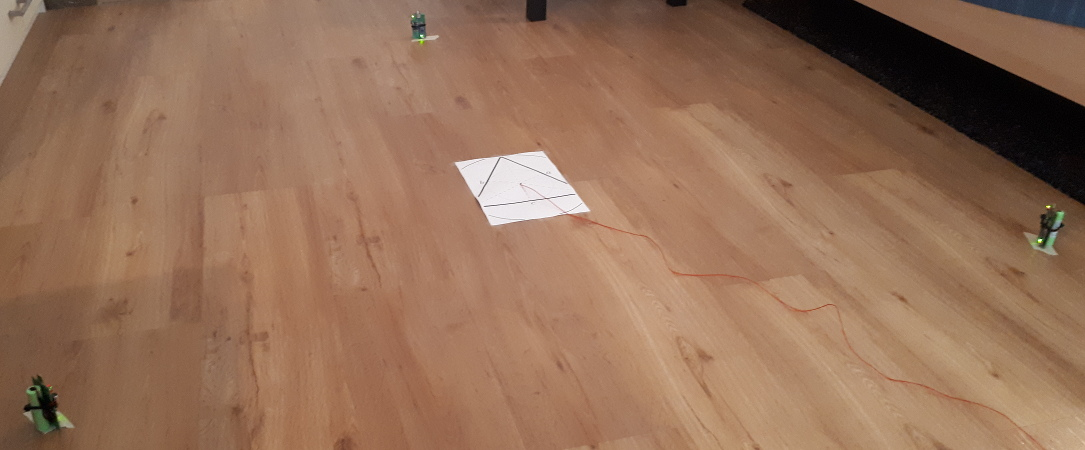
\includegraphics[width=0.9\linewidth]{calibration_triangle2}
	\caption{Versuchsaufbau für die Kalibierung von drei \Glsuseri{uwbm}.}
	\label{fig:calibration_triangle2}
\end{figure}

\begin{equation}
r_u = \frac{a}{3} \sqrt{3} \label{eq:dreieck_seitenlaenge_aus_umkreis}
\end{equation}

Initial wird die Antennenverzögerung bei allen \Glsuseri{uwbm} auf null gesetzt und danach reihum von jedem \Gls{uwbm} eintausend Entfernungsmessung zu den beiden benachbarten \Glsuseri{uwbm} durchgeführt. Insgesamt entstehen dabei sechstausend Datensätze, die mittels dem \textit{LGS}-- bzw. des \textit{DecaWave}--Kalibrierungsverfahren ausgewertet werden, siehe \autoref{tab:calibration_antenna_delay_results}

Das \textit{LGS}--Kalibrierungsverfahren lieferte für jeden Durchlauf reproduzierbare Ergebnisse. Da jedes \Gls{uwbm} herstellungsbedingte Unterschiede aufweist, ist es Plausibel das alle Antennenverzögerungen in einem ähnlichen Wertebereich liegen. Anders sieht es bei dem \textit{DecaWave}--Kalibrierungsverfahren aus. Hier ergeben sich für jeden Durchlauf andere Wertekombinationen, bedingt durch die Zufallskomponente bei der Erstellung der Kandidatenliste. Diese Verhalten von Genetischen--Algorithmen ist bekannt und muss daher bei der Auswahl der Wertekombinationen berücksichtigt werden. Am Beispiel der Spalte \textit{DecaWave 1} wird es sehr deutlich. Hier beträgt der Unterschied zwischen dem größten und kleinsten Wert \approx\SI{23}{\ns} und entspricht damit einer Abweichung von \approx\SI{6}{\meter} zwischen diesen beiden \Glsuseri{uwbm}.

\begin{table}[h]
	\centering
	\begin{tabular}{|c||c||c|c|c|c|}
\hline
\Gls{uwbm} & LGS [\si{\second}] & DecaWave [\si{\second}] & DecaWave 1 [\si{\second}] & DecaWave 2 [\si{\second}] \\
\hline\hline
176 & \num{257.45e9} & \num{242.48e9} & \num{232.21e9} & \num{254.50e9} \\
177 & \num{257.49e9} & \num{238.47e9} & \num{249.38e9} & \num{254.73e9} \\
178 & \num{257.11e9} & \num{257.17e9} & \num{255.36e9} & \num{215.07e9} \\

% Alte Darstellung
%176 & 16451 & 15494 & 14838 & 15912 & 16262 \\
%177 & 16453 & 15238 & 15935 & 15805 & 16277 \\
%178 & 16429 & 16433 & 16317 & 15131 & 13743 \\
\hline
	\end{tabular}
	\caption{Berechnete Werte für die Antennenverzögerung pro \Gls{uwbm}.}
	\label{tab:calibration_antenna_delay_results}
\end{table}

Die Wertekombinationen aus den Spalten \textit{LGS} und \textit{DecaWave} werden abwechselnd als Antennenverzögerungen in die \Glspl{uwbm} eingetragen und für jede Spalte jeweils eine weitere Messreihe, wie oben beschrieben, aufgezeichnet. Die Ergebnisse sind in der \autoref{tab:calibration_range_results} aufgeführt.

Mit einer initalen Antennenverzögerung von null beträgt der gemessene Abstand zwischen zwei \Glsuseri{uwbm} \approx \SI{156}{\meter} bei einem tatsächenlichen Abstand von \approx \SI{1.73}{\meter}. Eine Standardabweichung von \approx \SI{2}{\centi\meter} \footnote{Bei der Standardabweichung von über einem Meter handelt es sich um einen einzelnen Messfehler in der Messreihe.} entspricht dabei den Produkteigenschaften mit denen \textit{DecaWave} wirbt.

Werden die Antennenverzögerung aus der \textit{LGS}--Kalibrierungsverfahren benutzt, verbleibt die Standardabweichung in der gleichen Größenordnung wie im unkalibrierten Zustand. Jedoch nähert sich jetzt der gemessene Abstand dem tatsächlichen sehr stark an und bildet diesen sehr gut ab. Ganz im Gegensatz zu dem \textit{DecaWave}--Kalibrierungsverfahren.

\begin{table}[h]
	\centering
	\begin{tabular}{||c||c|c||ccccc||}
\hline
Kalibrierung & Tag & Anker & Entfernung & $\overline{x}_{arithm}$ & $\sigma$ & Min & Max \\\hline
Keine & 176 & 177 & \num{1.732} & \num{156.108} & \num{0.018} & \num{156.050} & \num{156.170} \\
Keine & 176 & 178 & \num{1.732} & \num{155.929} & \num{0.021} & \num{155.870} & \num{156.000} \\
Keine & 177 & 176 & \num{1.732} & \num{156.106} & \num{1.025} & \num{156.020} & \num{188.470} \\
Keine & 177 & 178 & \num{1.732} & \num{156.016} & \num{0.023} & \num{155.930} & \num{156.090} \\
Keine & 178 & 176 & \num{1.732} & \num{156.067} & \num{0.022} & \num{156.010} & \num{156.130} \\
Keine & 178 & 177 & \num{1.732} & \num{155.997} & \num{0.019} & \num{155.930} & \num{156.060} \\
\hline
LGS & 176 & 177 & \num{1.732} & \num{1.695} & \num{0.019} & \num{1.640} & \num{1.750} \\
LGS & 176 & 178 & \num{1.732} & \num{1.795} & \num{0.022} & \num{1.740} & \num{1.880} \\
LGS & 177 & 176 & \num{1.732} & \num{1.656} & \num{0.017} & \num{1.590} & \num{1.700} \\
LGS & 177 & 178 & \num{1.732} & \num{1.751} & \num{0.023} & \num{1.670} & \num{1.810} \\
LGS & 178 & 176 & \num{1.732} & \num{1.773} & \num{0.026} & \num{1.700} & \num{1.850} \\
LGS & 178 & 177 & \num{1.732} & \num{1.712} & \num{0.020} & \num{1.660} & \num{1.780} \\
\hline
DecaWave & 176 & 177 & \num{1.732} & \num{11.883} & \num{0.020} & \num{11.820} & \num{11.950} \\
DecaWave & 176 & 178 & \num{1.732} & \num{6.261} & \num{0.021} & \num{6.200} & \num{6.340} \\
DecaWave & 177 & 176 & \num{1.732} & \num{11.857} & \num{0.015} & \num{11.810} & \num{11.900} \\
DecaWave & 177 & 178 & \num{1.732} & \num{7.406} & \num{0.023} & \num{7.340} & \num{7.480} \\
DecaWave & 178 & 176 & \num{1.732} & \num{6.182} & \num{0.025} & \num{6.100} & \num{6.270} \\
DecaWave & 178 & 177 & \num{1.732} & \num{7.458} & \num{0.019} & \num{7.390} & \num{7.520} \\
\hline
	\end{tabular}
	\caption{Stochastische Eigenschaften der \Glspl{uwbm} ohne und mit Antennenkalibrierung bei einem Abstand von \SI{1.73}{\meter}.}
	\label{tab:calibration_range_results}
\end{table}



Im zweiten Kalibriervorgang werden alle fünf \Glspl{uwbm} eingeschlossen. Jetzt reicht ein Dreieck nicht mehr aus, statt dessen wird ein Pentagramm verwendet, siehe \autoref{fig:calibration_pentagram2}. Dieses lässt sich mathematisch ähnlich gut beschreiben wie das Dreieck. Aus der Seitenlänge $a = \SI{4.5}{\meter}$, zwischen zwei benachbarten Spitzen, wird über die \autoref{eq:pentagramm_diagonale} der Abstand $d$, zwischen den diagonalen Spitzen, berechnet. Der Umkreisradius $r_u$ ergibt sich aus der \autoref{eq:pentagramm_umkreisradius}.

\begin{equation}
d = \frac{a}{2} \left(1 + \sqrt{5} \right) \label{eq:pentagramm_diagonale}
\end{equation}

\begin{equation}
r_u = \frac{a}{10} \sqrt{50 + 10 \sqrt{5}} \label{eq:pentagramm_umkreisradius}
\end{equation}

\begin{figure}[h]
	\centering
	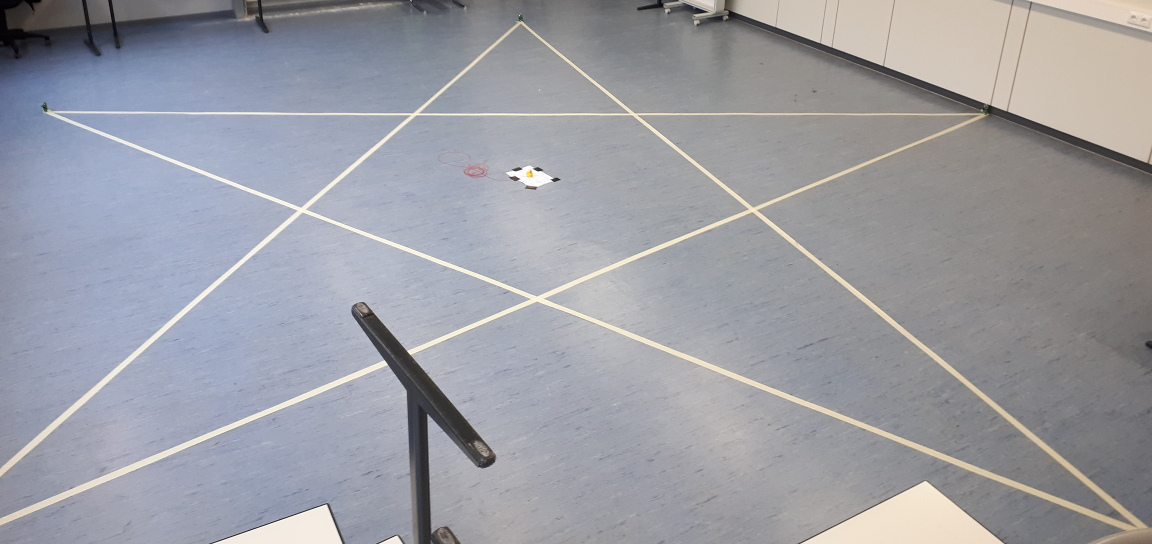
\includegraphics[width=0.9\linewidth]{calibration_pentagram2}
	\caption{Versuchsaufbau für die Kalibierung von fünf \Glsuseri{uwbm}.}
	\label{fig:calibration_pentagram2}
\end{figure}

Für das Pentagramm wurde nur noch das \textit{LGS}--Kalibrierungsverfahren verwendet, die Antennenverzögerungen pro \Gls{uwbm} sind dabei in der \autoref{tab:calibration_pentagramm_antenna_delay_results} aufgeführt.

\begin{table}[h]
	\centering
	\begin{tabular}{|c||c|}
\hline
\Gls{uwbm} & LGS [\si{\second}] \\
\hline\hline
176 & \num{257.30e9} \\
177 & \num{256.67e9} \\
178 & \num{256.67e9} \\
179 & \num{256.41e9} \\
180 & \num{257.20e9} \\

% Alte Darstellung
%176 & 16441 \\
%177 & 16401 \\
%178 & 16401 \\
%179 & 16384 \\
%180 & 16435 \\
\hline
	\end{tabular}
	\caption{Berechnete Werte für die Antennenverzögerung pro \Gls{uwbm} für das Pentagramm.}
	\label{tab:calibration_pentagramm_antenna_delay_results}
\end{table}




\begin{comment}
--------------------------------------------------------------------------------
- Mit welchen Einstellungen kommt man auf die Entfernungsmessung?
- Streuung?
- LOS/NLOS {Holz, Bücher, Menschlicher Körper}
	- Welcher Fehler ergibt zwischen LOS/NLOS?
- Wie verändert sich die Genauigkeit der Entfernungsmessung bei einer direkten Sichtverbindung (engl. Line--of--sight (LOS)) und indirekten Sichtverbindung (engl. Non--line--of--sight (NLOS))?
- isaacs2009optimal - Optimal sensor placement for time difference of arrival localization
- Diagramme
	- \cite{kurth2003experimental}
		- Fig. 2: Sample PDFs showing the true ranges associated with 20, 30, and 50 ft measured ranges. (X: true range, Y:count)
		- Fig. 3: The mean true distances to RF tags vs. measured distances (X:measured range, Y: true range)
		- Fig. 4: The variance in true distances to RF tags vs. measured distances (X:measured range (ft), Y: variance (ft^2))
	
- https://matheguru.com/stochastik/standardfehler.html
- https://de.wikipedia.org/wiki/Standardfehler

- Lichtgeschwindigkeit
	- https://de.wikipedia.org/wiki/Lichtgeschwindigkeit
	- In bodennaher Luft ist die Lichtgeschwindigkeit etwa 0,28 ‰ geringer als im Vakuum (also ca. 299.710 km/s), in Wasser beträgt sie etwa 225.000 km/s (−25 %) und in Gläsern mit hohem Brechungsindex bis hinab zu 160.000 km/s (−47 %).
	
\end{comment}
\section{Entfernungsmessung}

Um die Charakteristik der Entfernungsmessung zu bestimmen, wurde der Versuchsaufbau aus der \figurename~\ref{fig:entfernungsmessung_versuchsaufbau} verwendet. Dabei wird der \Gls{tag} an einem fixen Ort befestigt und die Entfernung zu dem \Gls{anchor} gemessen. Es wurden dabei acht Entfernungen mit einem Abstand von einem Meter gemessen. Zu jeder Entfernung wurden \num{249} Messungen aufgezeichnet. Die tatsächliche Entfernung wird mit einem Laser Entfernungsmesser, der eine Genauigkeit von $\pm$~\SI{2}{\milli\meter} besitzt, bestimmt.

\begin{figure}[ht!]
  \centering
  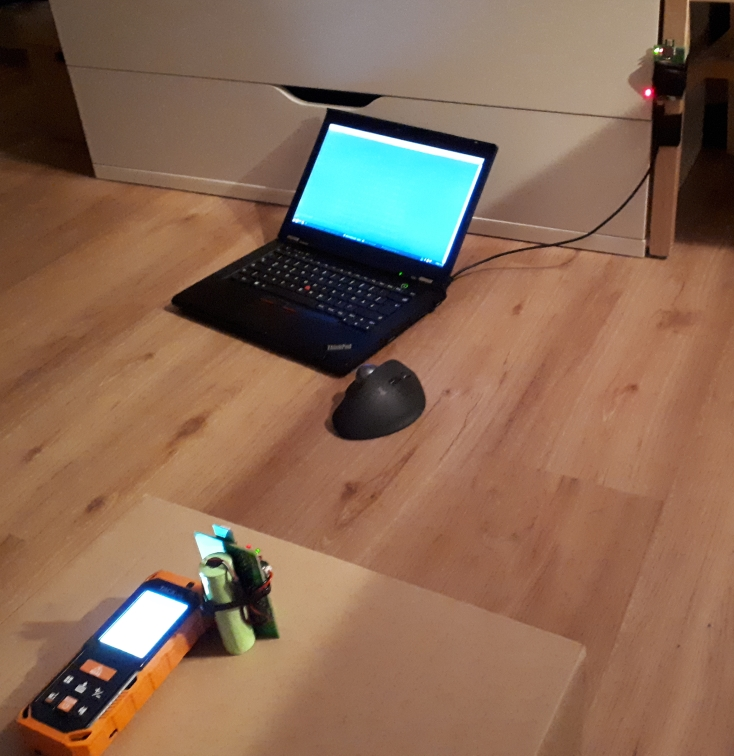
\includegraphics[width=0.5\linewidth]{entfernungsmessung_versuchsaufbau}
	\caption{Versuchsaufbau der Entfernungsmessung.}
	\label{fig:entfernungsmessung_versuchsaufbau}
\end{figure}

Die Ergebnisse der Entfernungsmessung können der \tablename~\ref{tab:entfernungsmessung_stochastik} entnommen werden. Auffällig sind die zum Teil großen Abweichung der Mittelwerte von der tatsächlichen Entfernungen, siehe Entfernung \SI{3}{\meter} und \SI{7}{\meter}. Mit \SI{10}{\centi\meter} sind die größten Ausreißer vom Mittelwert bei \SI{7}{\meter} zu verzeichnen. Die restlichen liegen im Bereich von \SIrange{4}{8}{\centi\meter}. Die Standardabweichung liegt mit \SI{3}{\centi\meter} in einem sehr guten Bereich, siehe auch \figurename~\ref{fig:entfernungsmessung_punktwolke}.

\begin{table}[h!]
	\centering
	\begin{tabular}{||c||c|c|c|c|c|c||}
		\hline
		Entfernung [\si{\meter}] & $\overline{x}_{arithm}$ & $\sigma$ & $\sigma^2$ & $SE_{\overline{x}}$ & Min & Max\\\hline
		\hline
		\num{1.00} & \num{1.0401} & \num{0.0298} & \num{0.0009} & \num{0.0019} & \num{0.96} & \num{1.12}\\\hline
		\num{2.00} & \num{2.0766} & \num{0.0164} & \num{0.0003} & \num{0.0010} & \num{2.03} & \num{2.12}\\\hline
		\num{3.00} & \num{3.1288} & \num{0.0218} & \num{0.0005} & \num{0.0014} & \num{3.07} & \num{3.18}\\\hline
		\num{4.00} & \num{3.9104} & \num{0.0221} & \num{0.0005} & \num{0.0014} & \num{3.86} & \num{3.97}\\\hline
		\num{5.00} & \num{5.0746} & \num{0.0383} & \num{0.0015} & \num{0.0024} & \num{5.00} & \num{5.19}\\\hline
		\num{6.00} & \num{6.0965} & \num{0.0177} & \num{0.0003} & \num{0.0011} & \num{6.05} & \num{6.16}\\\hline
		\num{7.00} & \num{7.1509} & \num{0.0324} & \num{0.0010} & \num{0.0021} & \num{7.08} & \num{7.25}\\\hline
		\num{8.00} & \num{7.9356} & \num{0.0191} & \num{0.0004} & \num{0.0012} & \num{7.89} & \num{7.98}\\\hline
	\end{tabular}
	\caption{Stochastische Eigenschaften der Entfernungsmessungen.}
	\label{tab:entfernungsmessung_stochastik}
\end{table}

\begin{figure}[h!]
  \centering
  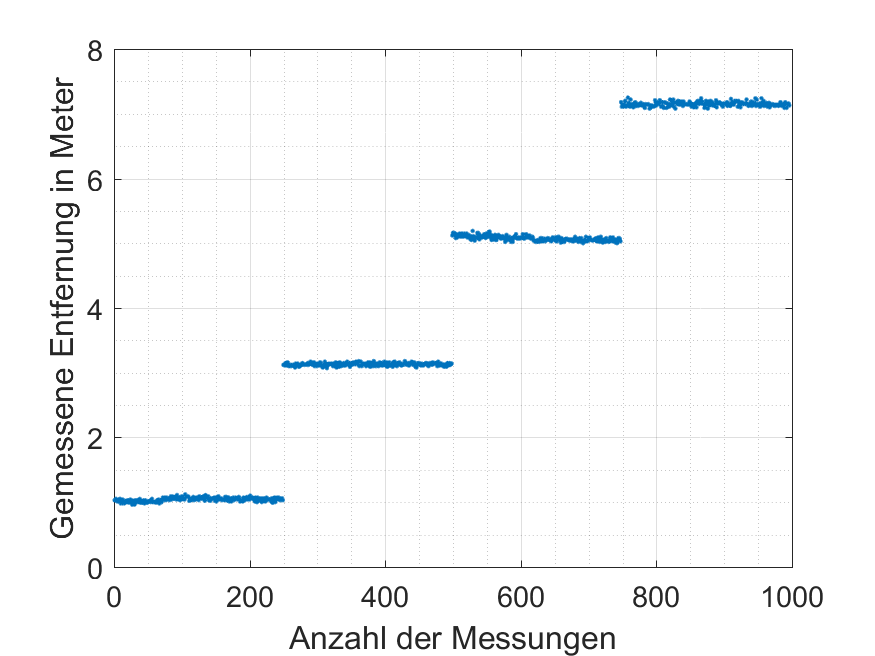
\includegraphics[width=0.5\linewidth]{entfernungsmessung_punktwolke}
	\caption{Verteilung der Messpunkte der ungeraden Entfernungsmessungen.}
	\label{fig:entfernungsmessung_punktwolke}
\end{figure}

In der \figurename~\ref{fig:entfernungsmessung_los_16440} wurden die ungeraden Entfernungsmessungen als Histogramm dargestellt. Gut zu erkennen ist die Normalverteilung der Messwerte um den Mittelwert.

\begin{figure}[h!]
	\centering
	\begin{subfigure}[b]{0.45\textwidth}
		\centering
		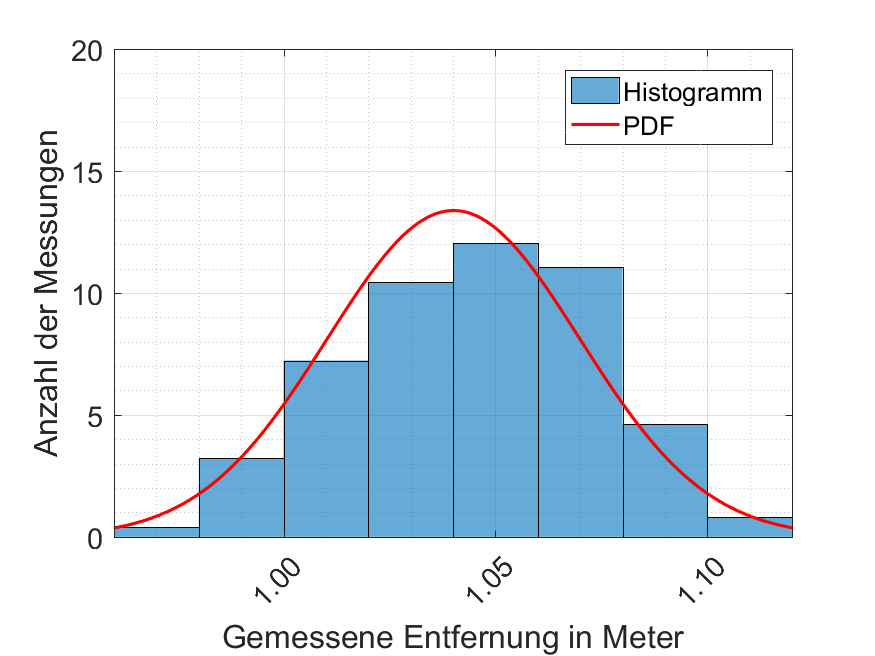
\includegraphics[width=\textwidth]{entfernungsmessung_los_1_16440}
		\caption{1 Meter}
		\label{fig:entfernungsmessung_los_1_16440}
	\end{subfigure}
	\hfill
	\begin{subfigure}[b]{0.45\textwidth}
		\centering
		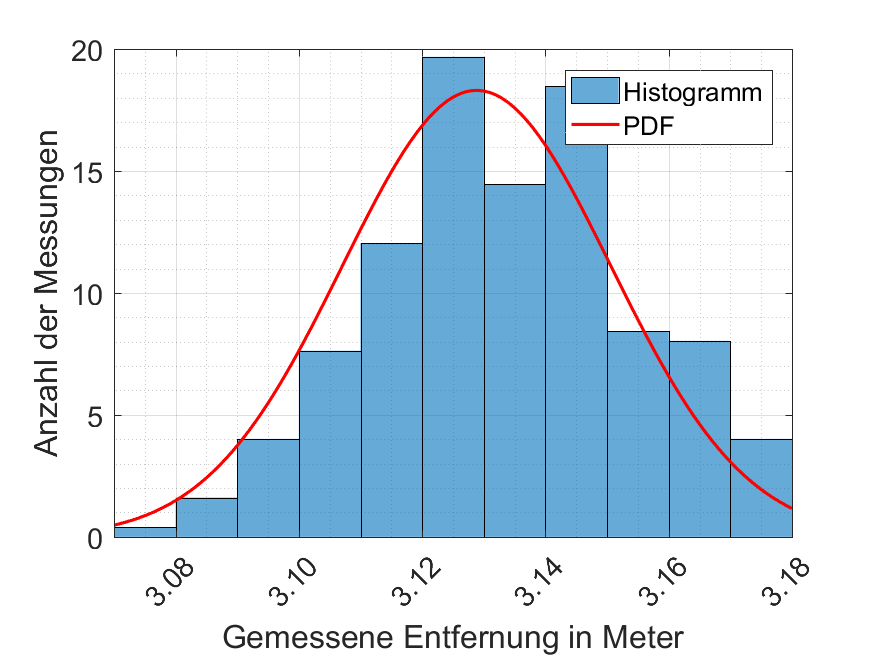
\includegraphics[width=\textwidth]{entfernungsmessung_los_3_16440}
		\caption{3 Meter}
		\label{fig:entfernungsmessung_los_3_16440}
	\end{subfigure}
	\bigskip
	\begin{subfigure}[b]{0.45\textwidth}
		\centering
		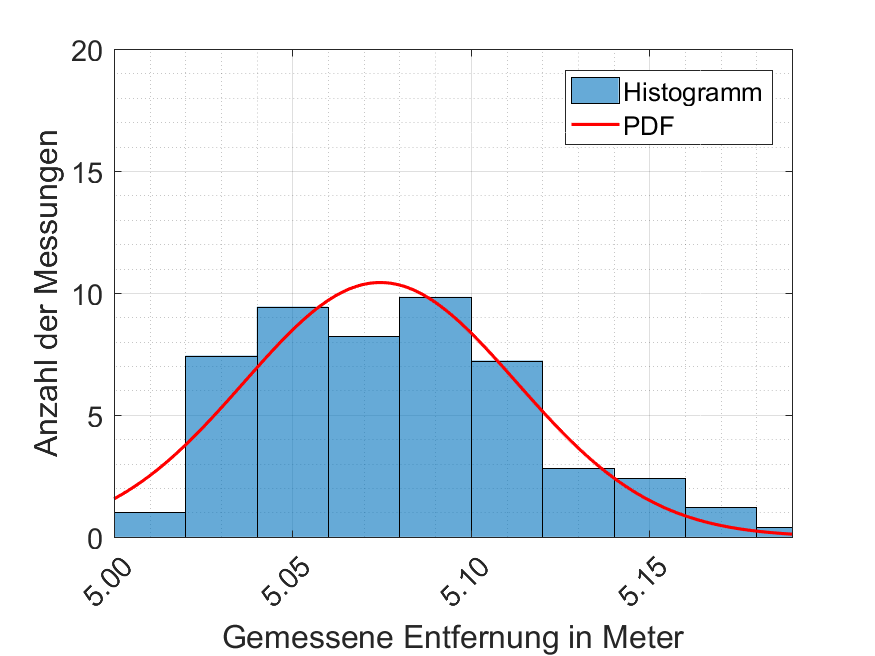
\includegraphics[width=\textwidth]{entfernungsmessung_los_5_16440}
		\caption{5 Meter}
		\label{fig:entfernungsmessung_los_5_16440}
	\end{subfigure}
	\hfil
	\begin{subfigure}[b]{0.45\textwidth}
		\centering
		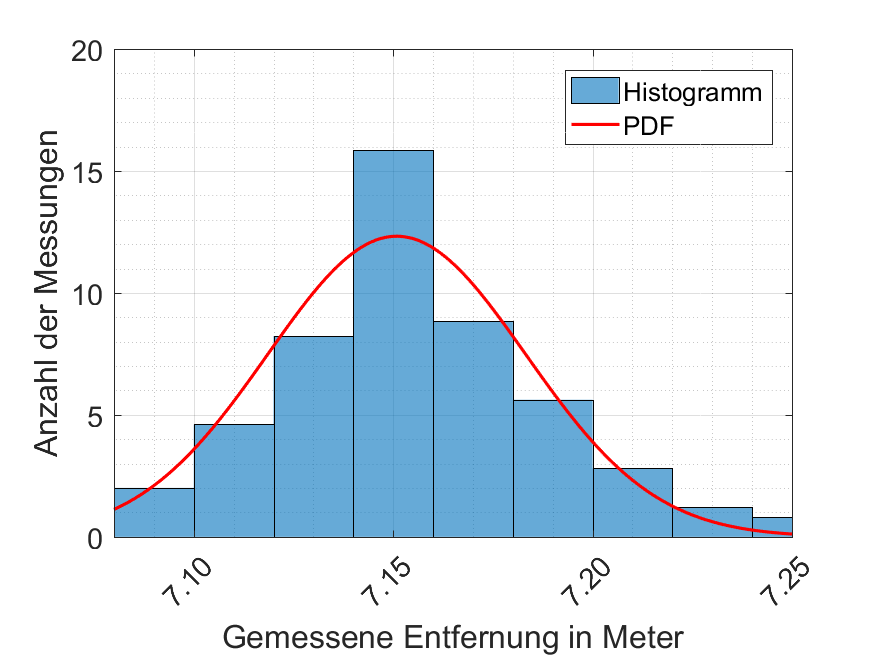
\includegraphics[width=\textwidth]{entfernungsmessung_los_7_16440}
		\caption{7 Meter}
		\label{fig:entfernungsmessung_los_7_16440}
	\end{subfigure}
	\caption{Histogramm und Wahrscheinlichkeitsdichtefunktion der ungeraden Entfernungsmessungen.}
	\label{fig:entfernungsmessung_los_16440}
\end{figure}


\begin{comment}
--------------------------------------------------------------------------------
- Diagramme
	- \cite{kurth2003experimental}
		- Fig. 5: (1) The ground truth path with tags indicated by circles. The numbers indicate how many range measurements were received from each tag over the duration of Test 1. (2) The path estimate from dead reckoning alone. (3) The path estimate from localization using a Kalman Filter. The Filter fuses data from odometry and a gyro with absolute measurements from RF tags to produce this path estimate. Numerical results are given in Table 1. (X: position in x(m), Y: position in y(m), Ground truth path with tag locations, Dead reckoning path, Kalman filter localization path)

		
- Versuchsbeschreibung:
	- Warum wurden die uwbm da platziert wo sie jetzt stehen?
	
\end{comment}
\section{RO-SLAM [todo]}


\begin{comment}
--------------------------------------------------------------------------------
\end{comment}
\subsection{Trajektorie [todo]}


\begin{comment}
--------------------------------------------------------------------------------
\end{comment}
\subsection{Vergleich von MC und SOG [todo]}

